%%%%%%%%%%%%%%%%%%%%%%%%%%%%%%%

\section{Invariant $B$ mass fit and Dalitz plot distributions} 
\label{sec:MassFit}

After the selections, 
the sample of $\LbJpsiPPi$ decays consists of the signal, 
the combinatorial background and the \LbJpsipK relections.
The invariant mass distribution of the signal is described by a DSCB function, 
an alternative fit with the Hypatia model is also performed; 
the shape of the combinatorial background is described by an exponential function; 
and the shapes of the \LbJpsipK reflections are determined from simulation.  
A simulation $\LbJpsipK$ sample is used to determine the shapes of the reflections. 
The candidate is reconstructed as $\Lb\to\jpsi\proton[\Km\to\pim]$, 
and all selections except the PID requirements used to select $\LbJpsiPPi$ candidates in this analysis are applied to these candidates. 
Each event that passes the selections is assigned a weight to account for the PID efficiency, 
and the weight is determined from the PIDCalib package. 
By filling the invariant mass under $\jpsi\proton\pim$ hypotheses into histograms with the PID weight, 
the shapes are determined,
as shown in Fig.~\ref{fig:MisIDLb2JpsiPK}. 
The histogram is converted to a histogram-PDF in the fit. 
It should be noted that the shape is found to be insensitive to the decay model\,
\footnote{The shape determined in different slices of $M(p\pi)$ is very similar.}, 
so the shape determined from the simulation with the PHSP decay model
is good enough to represent the complicated Dalitz distribution seen in the data. 

In Figure.~\ref{fig:MassFit}, 
the fitted invariant mass distributions of the $\LbJpsiPPi$ candidate are shown for both Run 1 and Run 2 samples. 
The signal yields given by the fit are $1960\pm53$ for Run1 and $8607\pm111$ for Run2, 
%and the total number of the \LbJpsipK reflections is $1033\pm150$. 
The $\jpsi p\pi^-$ signal peak has a mean value of $5620.1\pm0.1\mevcc$.

The invariant mass fit result is used to calculate the \sWeights for both the signal and background components. 
%The signal \sWeights are used to subtract the background.
In Figure.~\ref{fig:dlz}, 
the ``Dalitz" plots using the invariant mass squared are shown, 
$m^2_{p\pim}$ vs $m^2_{\jpsi\proton}$,  and $m^2_{p\pim}$ vs $m^2_{\jpsi\pi}$ as independent variables. 
Here,
the Run 1 and Run 2 are put together.
As expected, 
significant $N^{*}$ contributions are seen, 
especially in the region around $m^2{p\pim}=2\gevgevcccc$.
It seems that narrow belt around the $P_c(4450)$ region at about $20\gevgevcccc$ in the $\jpsi p$ mass-squared is visible.
While many events concentrate in a limited window around $m^2_{p\pi} = 6\gevgevcccc$ and $m^2_{\jpsi p}$ between $18$ to $20\gevgevcccc$, 
which could be due to the $P_c$ contribution. 
These events are also presented at the region of $m^2_{\jpsi \pim}$ around 17$\gevgevcccc$ with $m^2_{p\pi}$ around 6$\gevgevcccc$.
%The projections of the $p\pim$ and $\jpsi p$ invariant masses are displayed in Fig.~\ref{mproj}. 
%For completeness, we show the distributions of efficiency and background on the Dalitz plane in Fig.~\ref{dlzbg}, 
%where the background is the events from the mass sideband of $5665-5770$\mev. 
%Appendix~\ref{Sideband} shows the mass spectra of any two final state combinations for both low and high sidebands.


%%%%%%%%%%%%%%%%%%%%%%%%%%%%%%%%%%%%%%%%%%%%%%%%%%%%%%%%%%%%%%%%%%%%%%%%%%%%%%%%%%%%%%%%%%%%%%%%%%%%%%%%%%%%%%%%%%%%%%%
\begin{figure}[!tbh]
\centering
\begin{minipage}[t]{0.5\textwidth}
\centering
   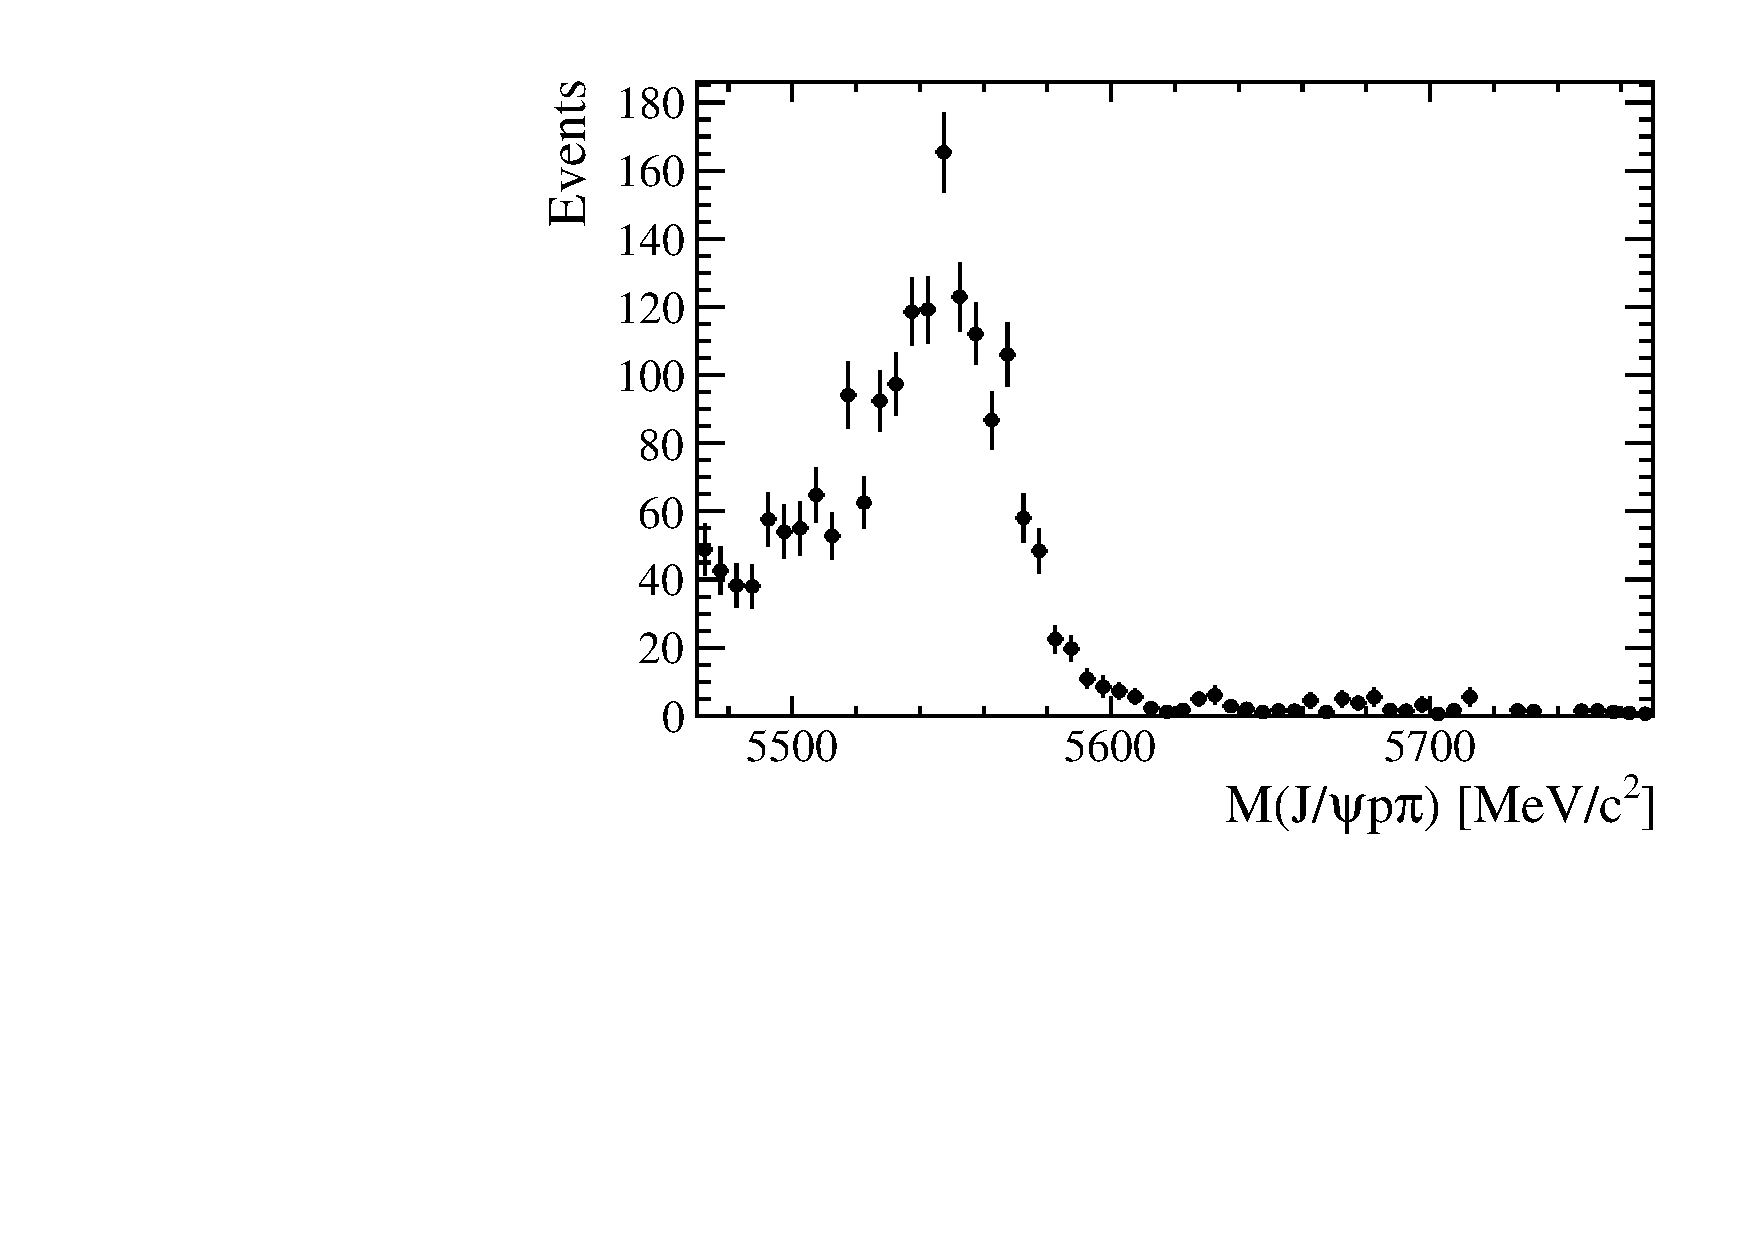
\includegraphics[width=1.0\textwidth]{Figures/04_Penta/03_mass_fit/phy_bkg.pdf}
\put(-70,100) {\textrm{\small \bf Unofficial}} 
\end{minipage}
\caption{Distribution of the invariant mass of \LbJpsipK candidates reconstructed as \LbJpsippi.} 
\label{fig:MisIDLb2JpsiPK}
\end{figure}
%%%%%%%%%%%%%%%%%%%%%%%%%%%%%%%%%%%%%%%%%%%%%%%%%%%%%%%%%%%%%%%%%%%%%%%%%%%%%%%%%%%%%%%%%%%%%%%%%%%%%%%%%%%%%%%%%%%%%%%


%%%%%%%%%%%%%%%%%%%%%%%%%%%%%%%%%%%%%%%%%%%%%%%%%%%%%%%%%%%%%%%%%%%%%%%%%%%%%%%%%%%%%%%%%%%%%%%%%%%%%%%%%%%%%%%%%%%%%%%
\begin{figure}[!tbh]
\centering
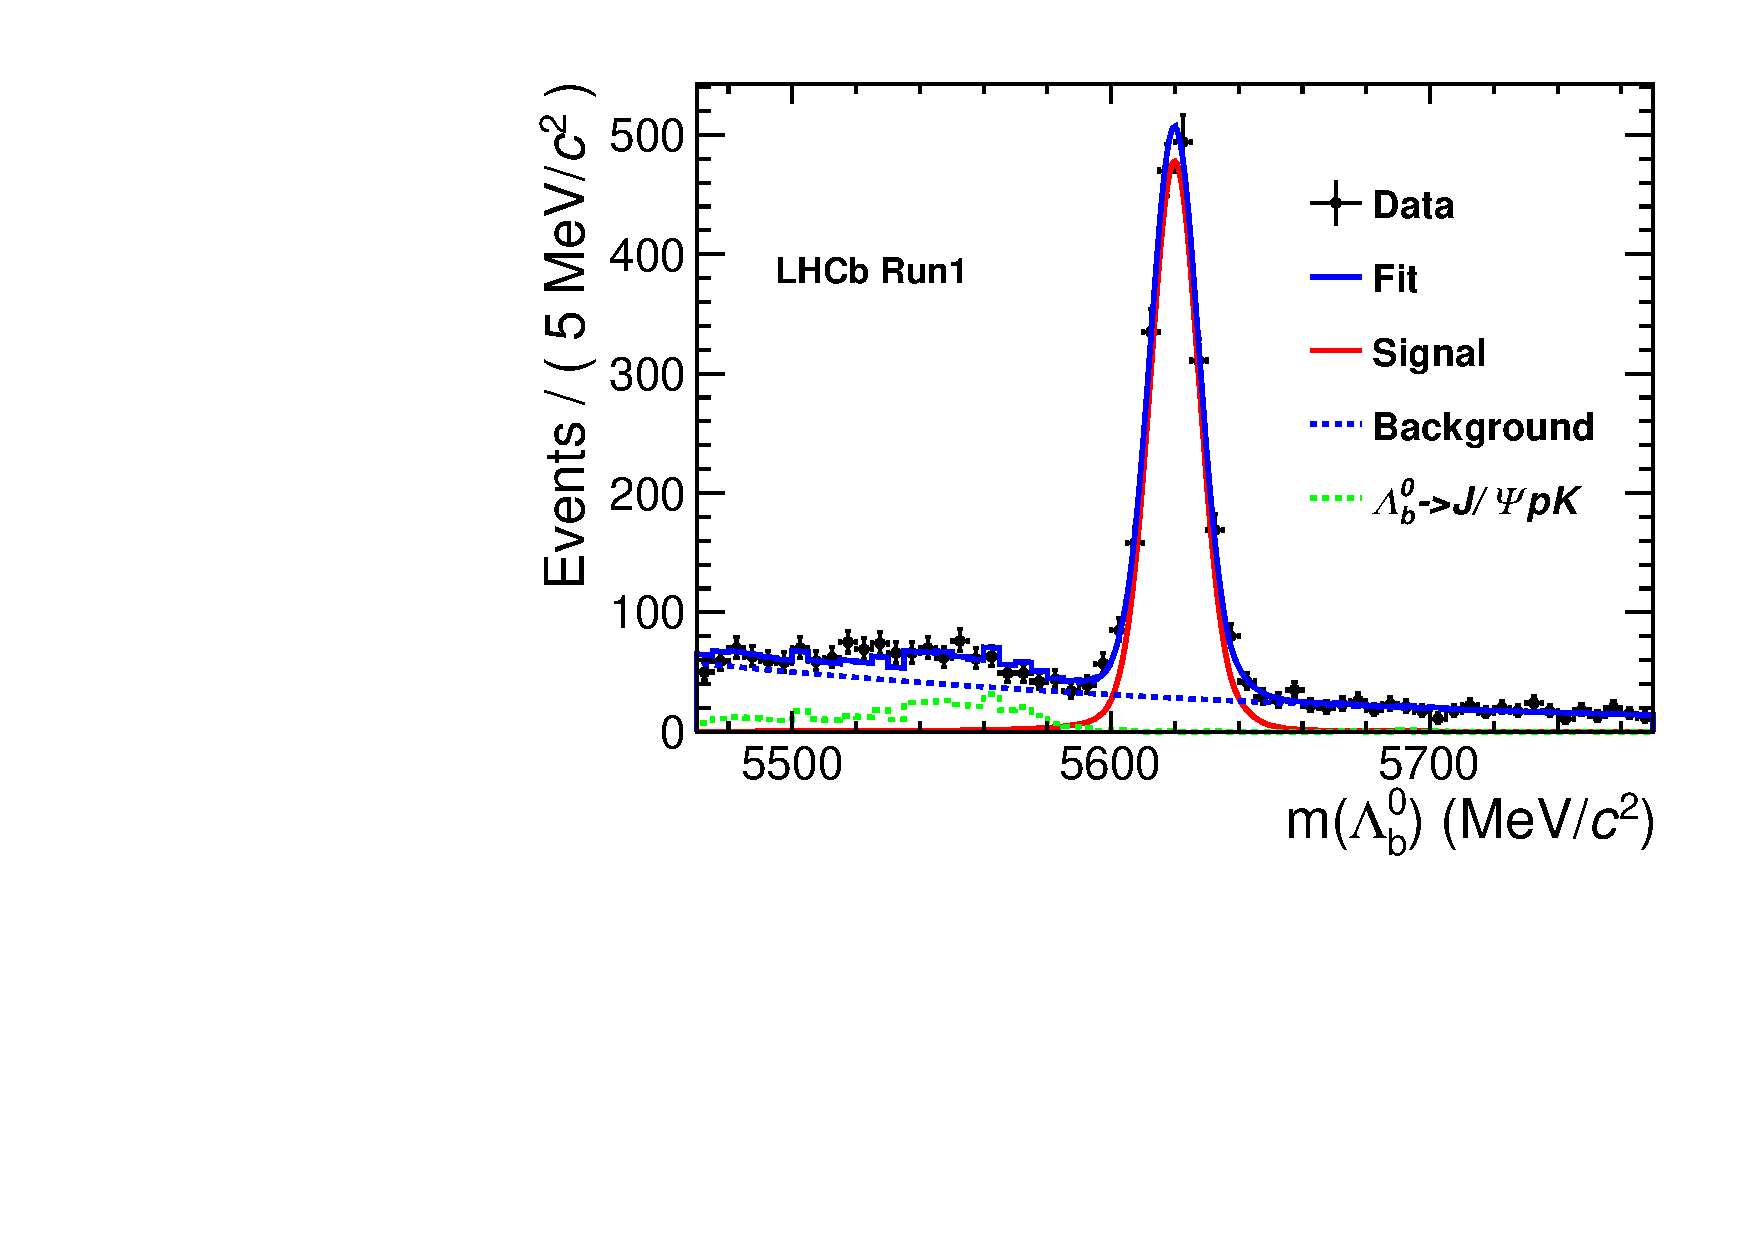
\includegraphics[width=0.49\textwidth]{Figures/04_Penta/03_mass_fit/Lb_Jpsippi_run1}
\put(-170,90) {\textrm{\small \bf Unofficial}} 
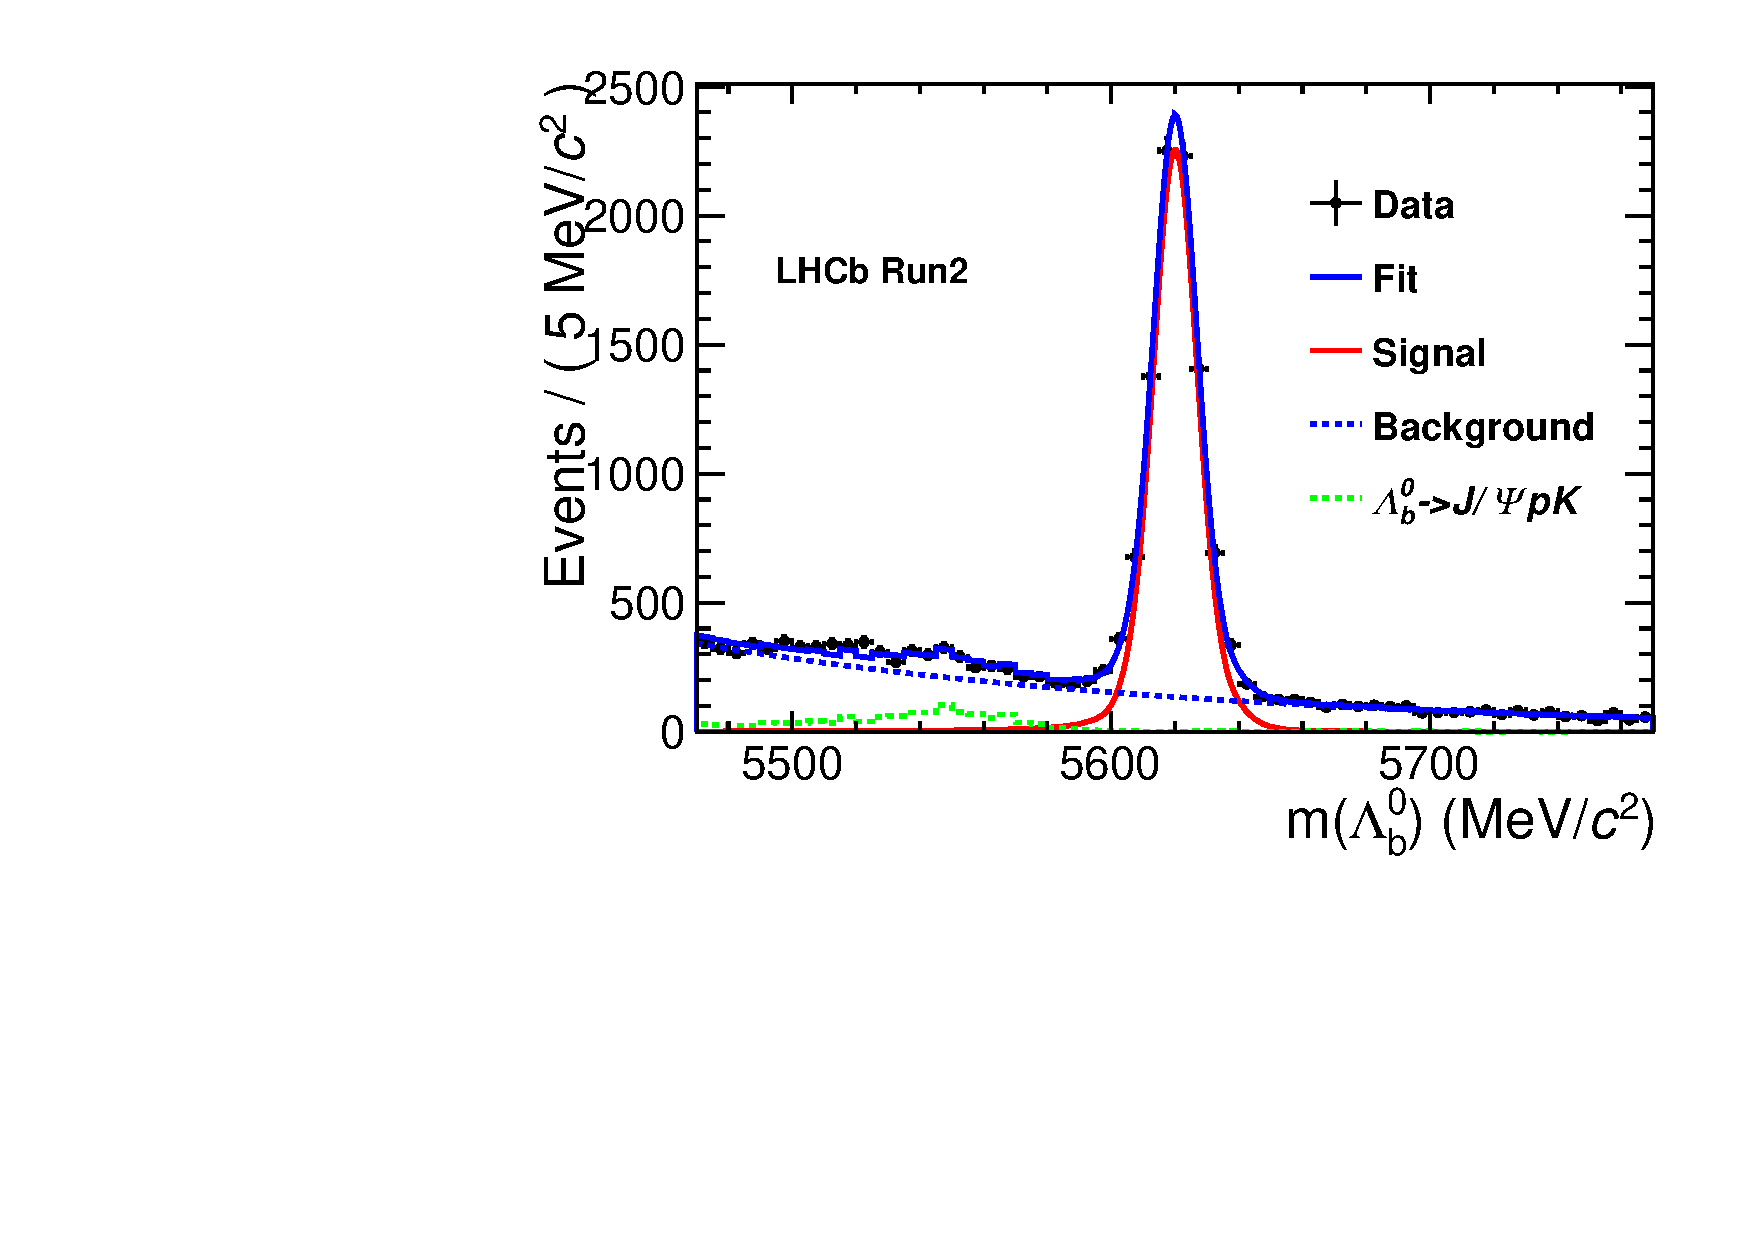
\includegraphics[width=0.49\textwidth]{Figures/04_Penta/03_mass_fit/Lb_Jpsippi_run2}
\put(-170,90) {\textrm{\small \bf Unofficial}} 
   \caption{Invariant mass distribution of the $\LbJpsiPPi$ decay and the fitted curve for Run 1(left) and Run 2(right) samples.} 
\label{fig:MassFit}
\end{figure}
%%%%%%%%%%%%%%%%%%%%%%%%%%%%%%%%%%%%%%%%%%%%%%%%%%%%%%%%%%%%%%%%%%%%%%%%%%%%%%%%%%%%%%%%%%%%%%%%%%%%%%%%%%%%%%%%%%%%%%%



%%%%%%%%%%%%%%%%%%%%%%%%%%%%%%%%%%%%%%%%%%%%%%%%%%%%%%%%%%%%%%%%%%%%%%%%%%%%%%%%%%%%%%%%%%%%%%%%%%%%%%%%%%%%%%%%%%%%%%%
\begin{figure}[!tbh]
\centering
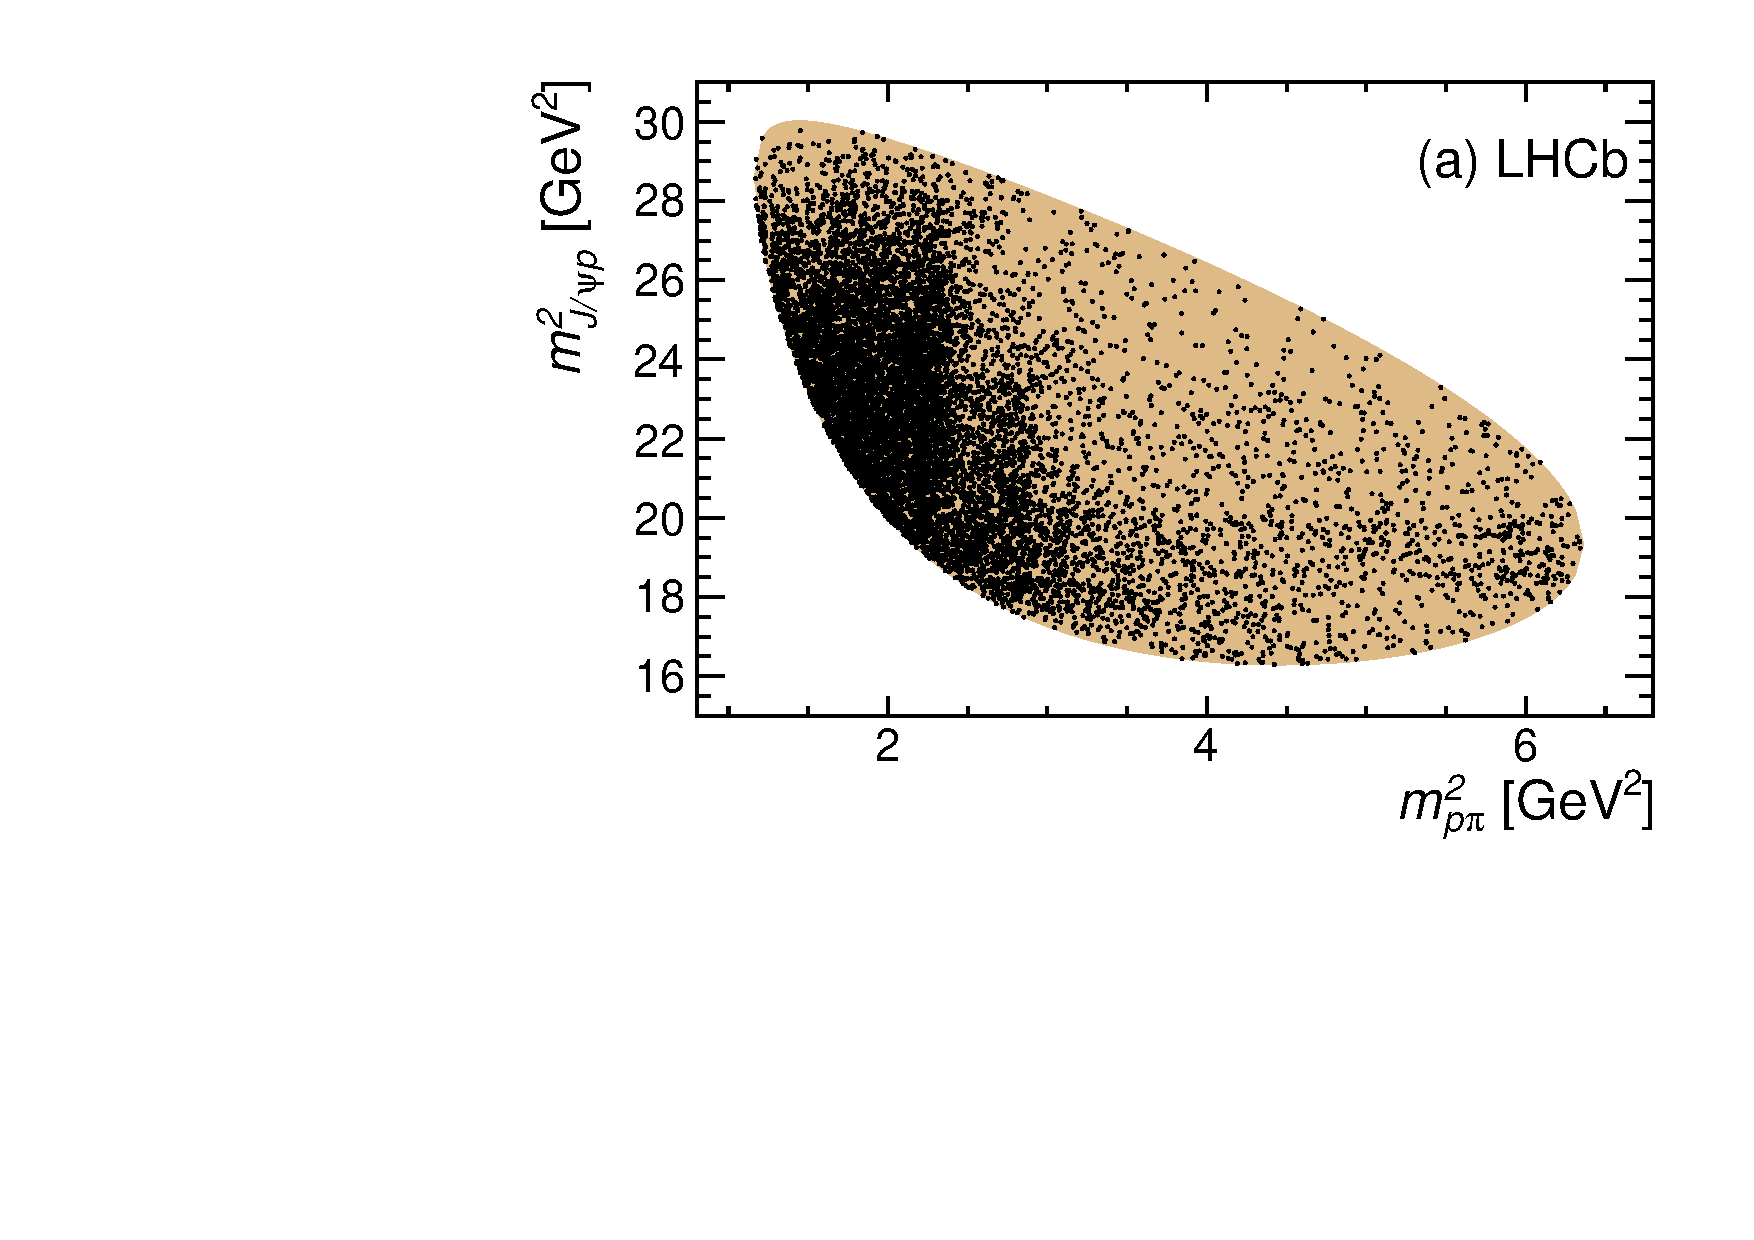
\includegraphics[width=0.65\textwidth]{Figures/04_Penta/03_mass_fit/dlz-point} 
\put(-70,145) {\textrm{\normalsize \bf Unofficial}} 
\\
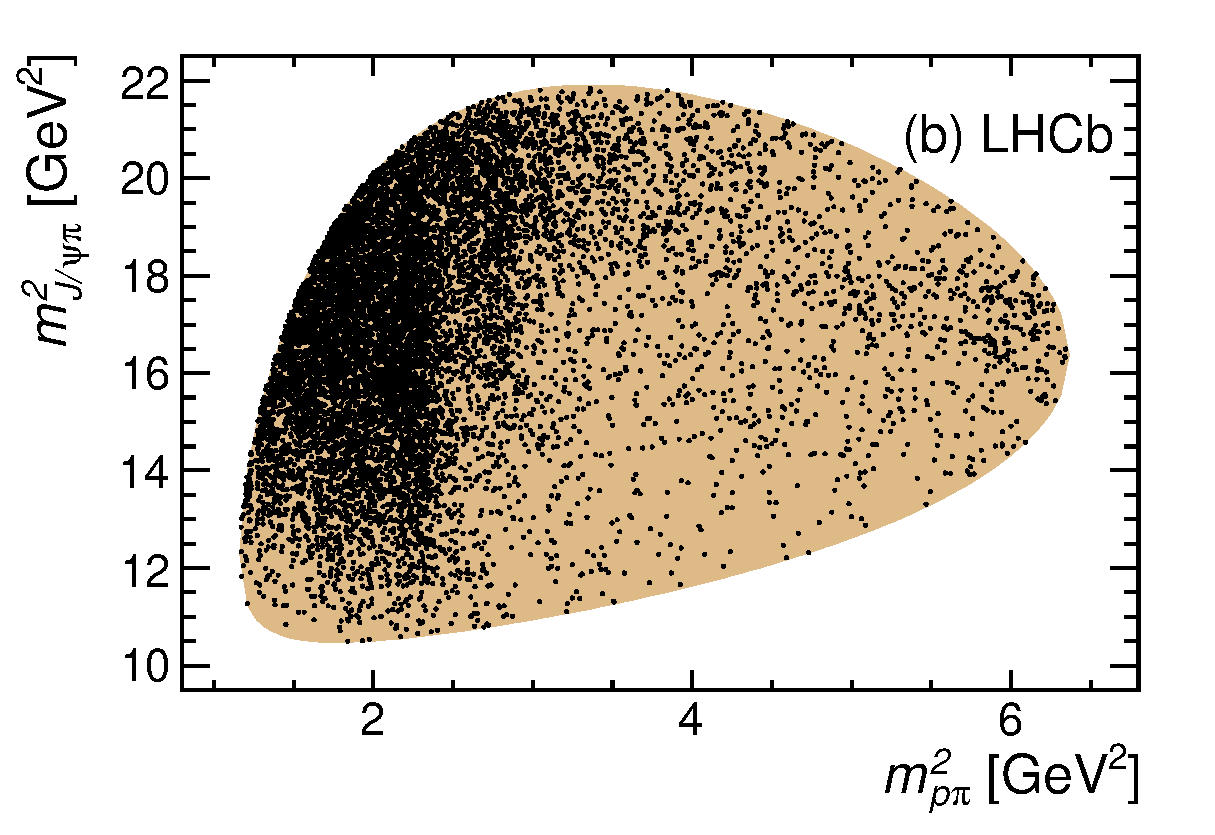
\includegraphics[width=0.65\textwidth]{Figures/04_Penta/03_mass_fit/dlzk-point}
\put(-70,50) {\textrm{\normalsize \bf Unofficial}} 
\caption{Invariant mass squared of $\proton\pi$ versus either $\jpsi\proton$ (top) or $\jpsi\pi$ (bottom) for candidates 
   with \sWeights to subtract background contribution. 
   The hatched area shows the kinematic allowed region.} 
\label{fig:dlz}
\end{figure}
%%%%%%%%%%%%%%%%%%%%%%%%%%%%%%%%%%%%%%%%%%%%%%%%%%%%%%%%%%%%%%%%%%%%%%%%%%%%%%%%%%%%%%%%%%%%%%%%%%%%%%%%%%%%%%%%%%%%%%%




